%%%%%%%%%%%%%%%%%%%%%%%%%%
%%% author : Yamada. T %%%
%%% made for TH series %%%
%%%%%%%%%%%%%%%%%%%%%%%%%%

\documentclass[b5paper,10pt,fleqn] {ltjsarticle}

\usepackage[margin=10truemm]{geometry}

\usepackage{pict2e, graphicx}
\usepackage{tikz}
\usetikzlibrary{intersections,calc,arrows.meta}

\usepackage{amsmath, amssymb, amsthm}
\usepackage{ascmac}
\usepackage{comment}
\usepackage{empheq}
\usepackage[shortlabels,inline]{enumitem}
\usepackage{fancybox}
\usepackage{fancyhdr}
\usepackage{here}
\usepackage{lastpage}
\usepackage{listings, jvlisting}
\usepackage{fixdif}

\usepackage{stmaryrd}
\usepackage[listings]{tcolorbox}
%\usepackage{ascolorbox}
\usepackage{titlesec}
\usepackage{ulem}
\usepackage{url}
\usepackage{verbatim}
\usepackage{wrapfig}
\usepackage{xcolor}
\usepackage{luatexja-ruby}
\usepackage{varwidth}
\usepackage[version=3]{mhchem}
\usepackage{wrapfig}


\usepackage{physics2}
	\usephysicsmodule{ab}
	\usephysicsmodule{ab.braket}
	\usephysicsmodule{ab.legacy}
	%\usephysicsmodule{braket}
	\usephysicsmodule{diagmat}
	\usephysicsmodule{xmat}
	\usephysicsmodule{nabla.legacy}
	\usephysicsmodule{qtext.legacy}

\usepackage[ISO]{diffcoeff}
\difdef { f, s } { D }
{ op-symbol = \mathrm{D} }


\newcommand{\mctext}[1]{\mbox{\textcircled{\scriptsize{#1}}}}
\newcommand{\ctext}[1]{\textcircled{\scriptsize{#1}}}
\newcommand{\ds}{\displaystyle}
\newcommand{\comb}[2]{{}_{#1}\mathrm{C}_{#2}}
\newcommand{\hs}{\hspace}
\newcommand{\vs}{\vspace}
\newcommand{\emphvs}{\vspace{1em}\notag\\}
\newcommand{\ora}{\overrightarrow}
\newcommand{\ol}{\overline}
\newcommand{\oramr}[1]{\overrightarrow{\mathrm{#1}}}
\newcommand{\tri}{\triangle}
\newcommand{\mr}{\mathrm}
\newcommand{\mb}{\mathbb}
\newcommand{\mrvec}[1]{\overrightarrow{\mathrm{#1}}}
\newcommand{\itvec}{\overrightarrow}
\newcommand{\bs}{\boldsymbol}
\newcommand{\ra}{\rightarrow}
\newcommand{\Ra}{\Rightarrow}
\newcommand{\lra}{\longrightarrow}
\newcommand{\Lra}{\Longrightarrow}
\newcommand{\la}{\leftarrow}
\newcommand{\La}{\Leftarrow}
\newcommand{\lla}{\longleftarrow}
\newcommand{\Lla}{\Longleftarrow}
\newcommand{\lr}{\leftrightarrow}
\newcommand{\llr}{\longleftrightarrow}
\newcommand{\Llr}{\Longleftrightarrow}
\renewcommand{\deg}{{}^\circ}
\newcommand{\phbox}{\fbox{\phantom{1\hspace{2em}}}}
\newcommand{\boxnum}[1]{\fbox{\phantom{\hspace{1em}}({#1})\phantom{\hspace{1em}}}}
\newcommand{\boxkana}[1]{\fbox{\phantom{\hspace{1em}}{#1}\phantom{\hspace{1em}}}}
\newcommand{\boxkm}[2]{\fbox{\, {#1}\phantom{\hspace{0.2em}} \,  {#2}}}
\newcommand{\hzw}{\hspace{1\zw}}

\renewcommand{\baselinestretch}{1.25}
\parindent=1\zw

%入86
\begin{document}
\noindent
\fbox{NewTH1-8} [東京大]

%\begin{wrapfigure}{r}{6cm}
%  \centering
%  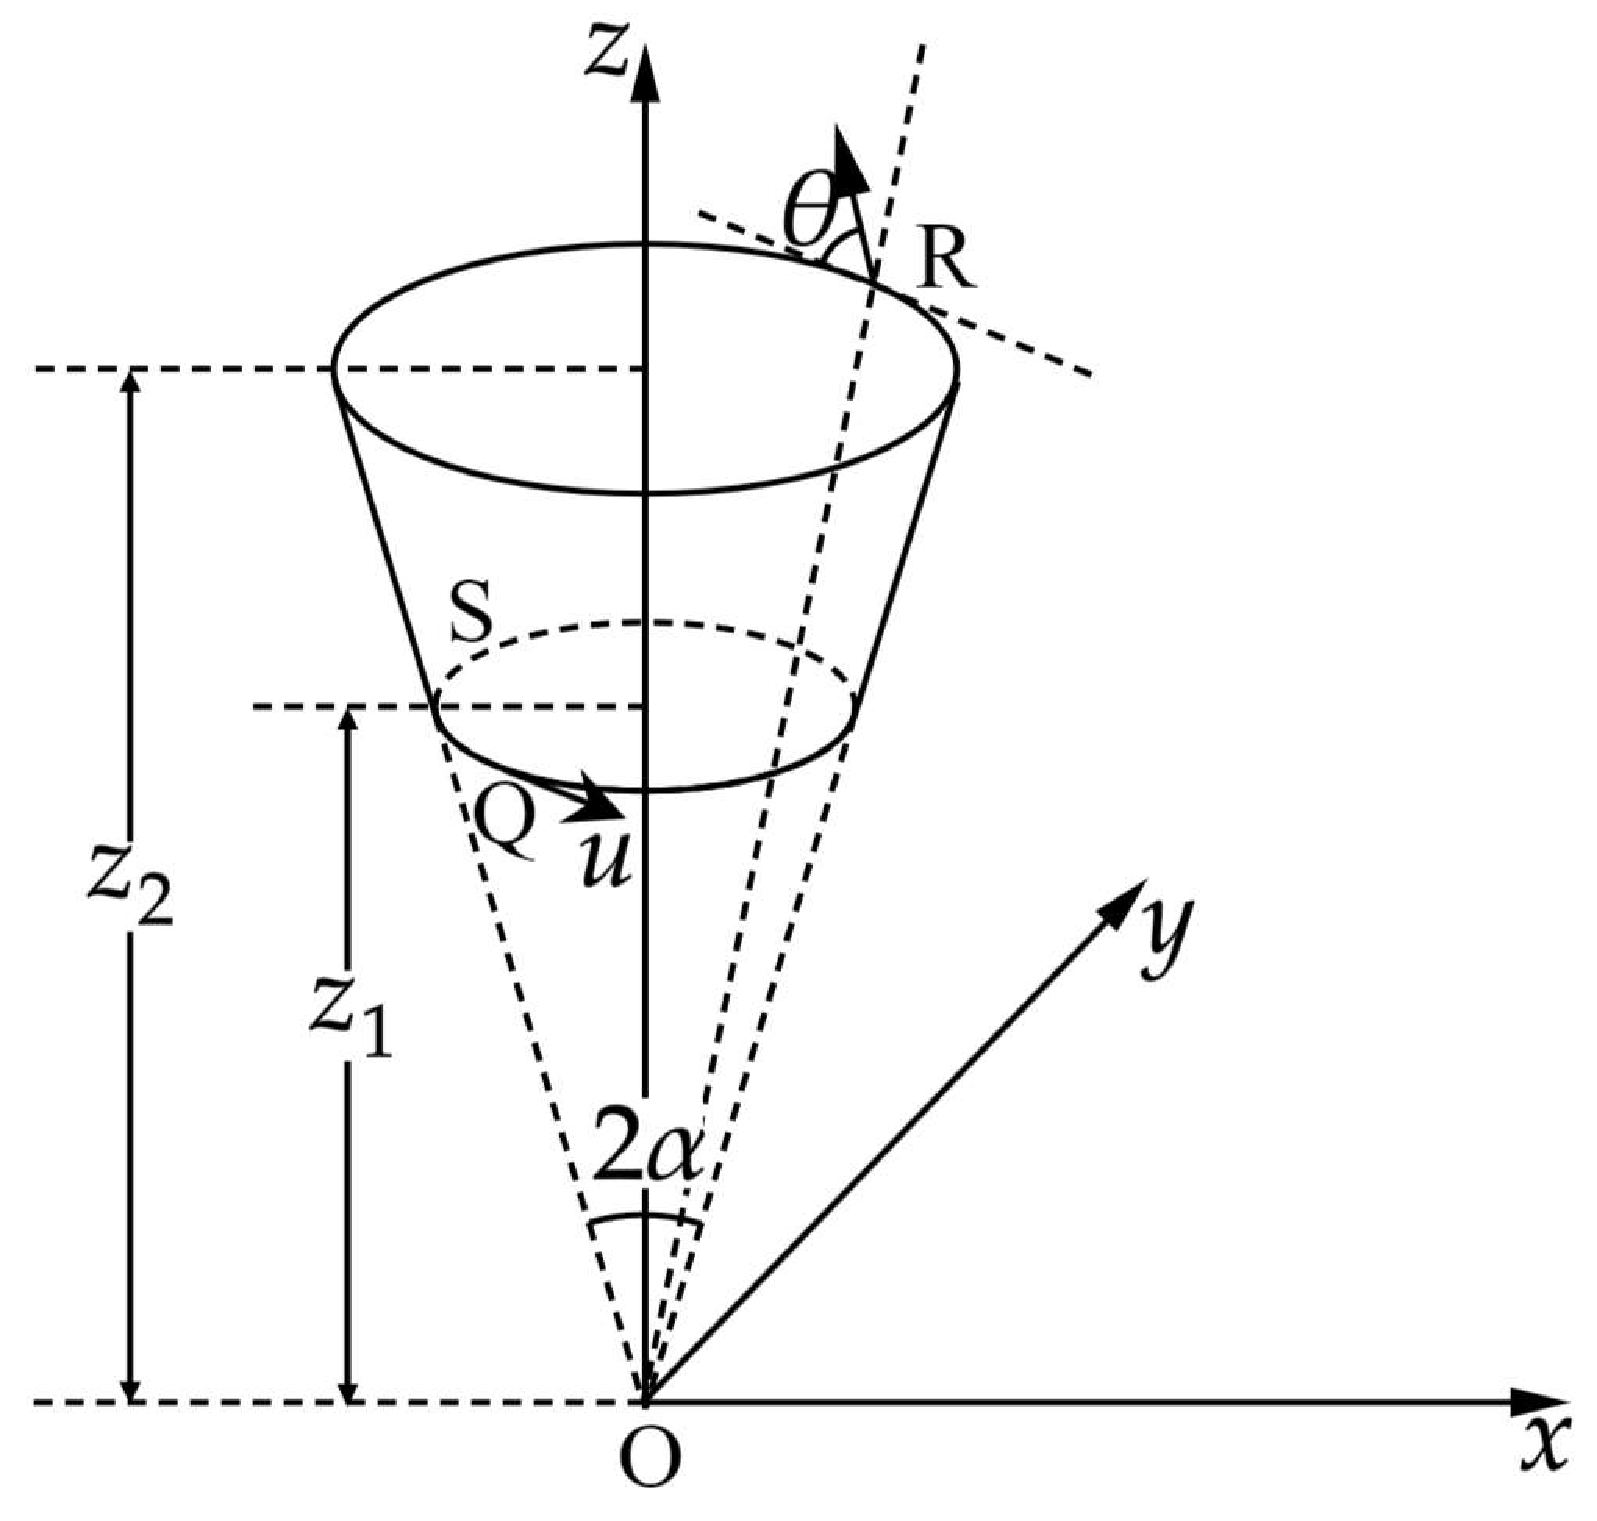
\includegraphics[width=6cm]{fig/fig_1_8.pdf}
%\end{wrapfigure}

図のように曲面Sは2つの水平面によって切り取られた円錐側面の一部である.この面の内側に沿って運動する質量$m$の質点を考える.

円錐の頂角は$2 \alpha$であり,円錐の軸は鉛直方向であるとする.頂点Oを原点にとり,水平面内に$x$軸と$y$軸を,鉛直上向きに$z$軸をとる.Sの下端の$z$座標は$z_1$,上端の$z$座標は$z_2$であり,その範囲を超えると質点は自由に運動できる.Sと質点の間の摩擦は無視できるものとし,重力加速度の大きさを$g$として,以下の設問に答えよ.

\begin{figure}[H]
  \centering
  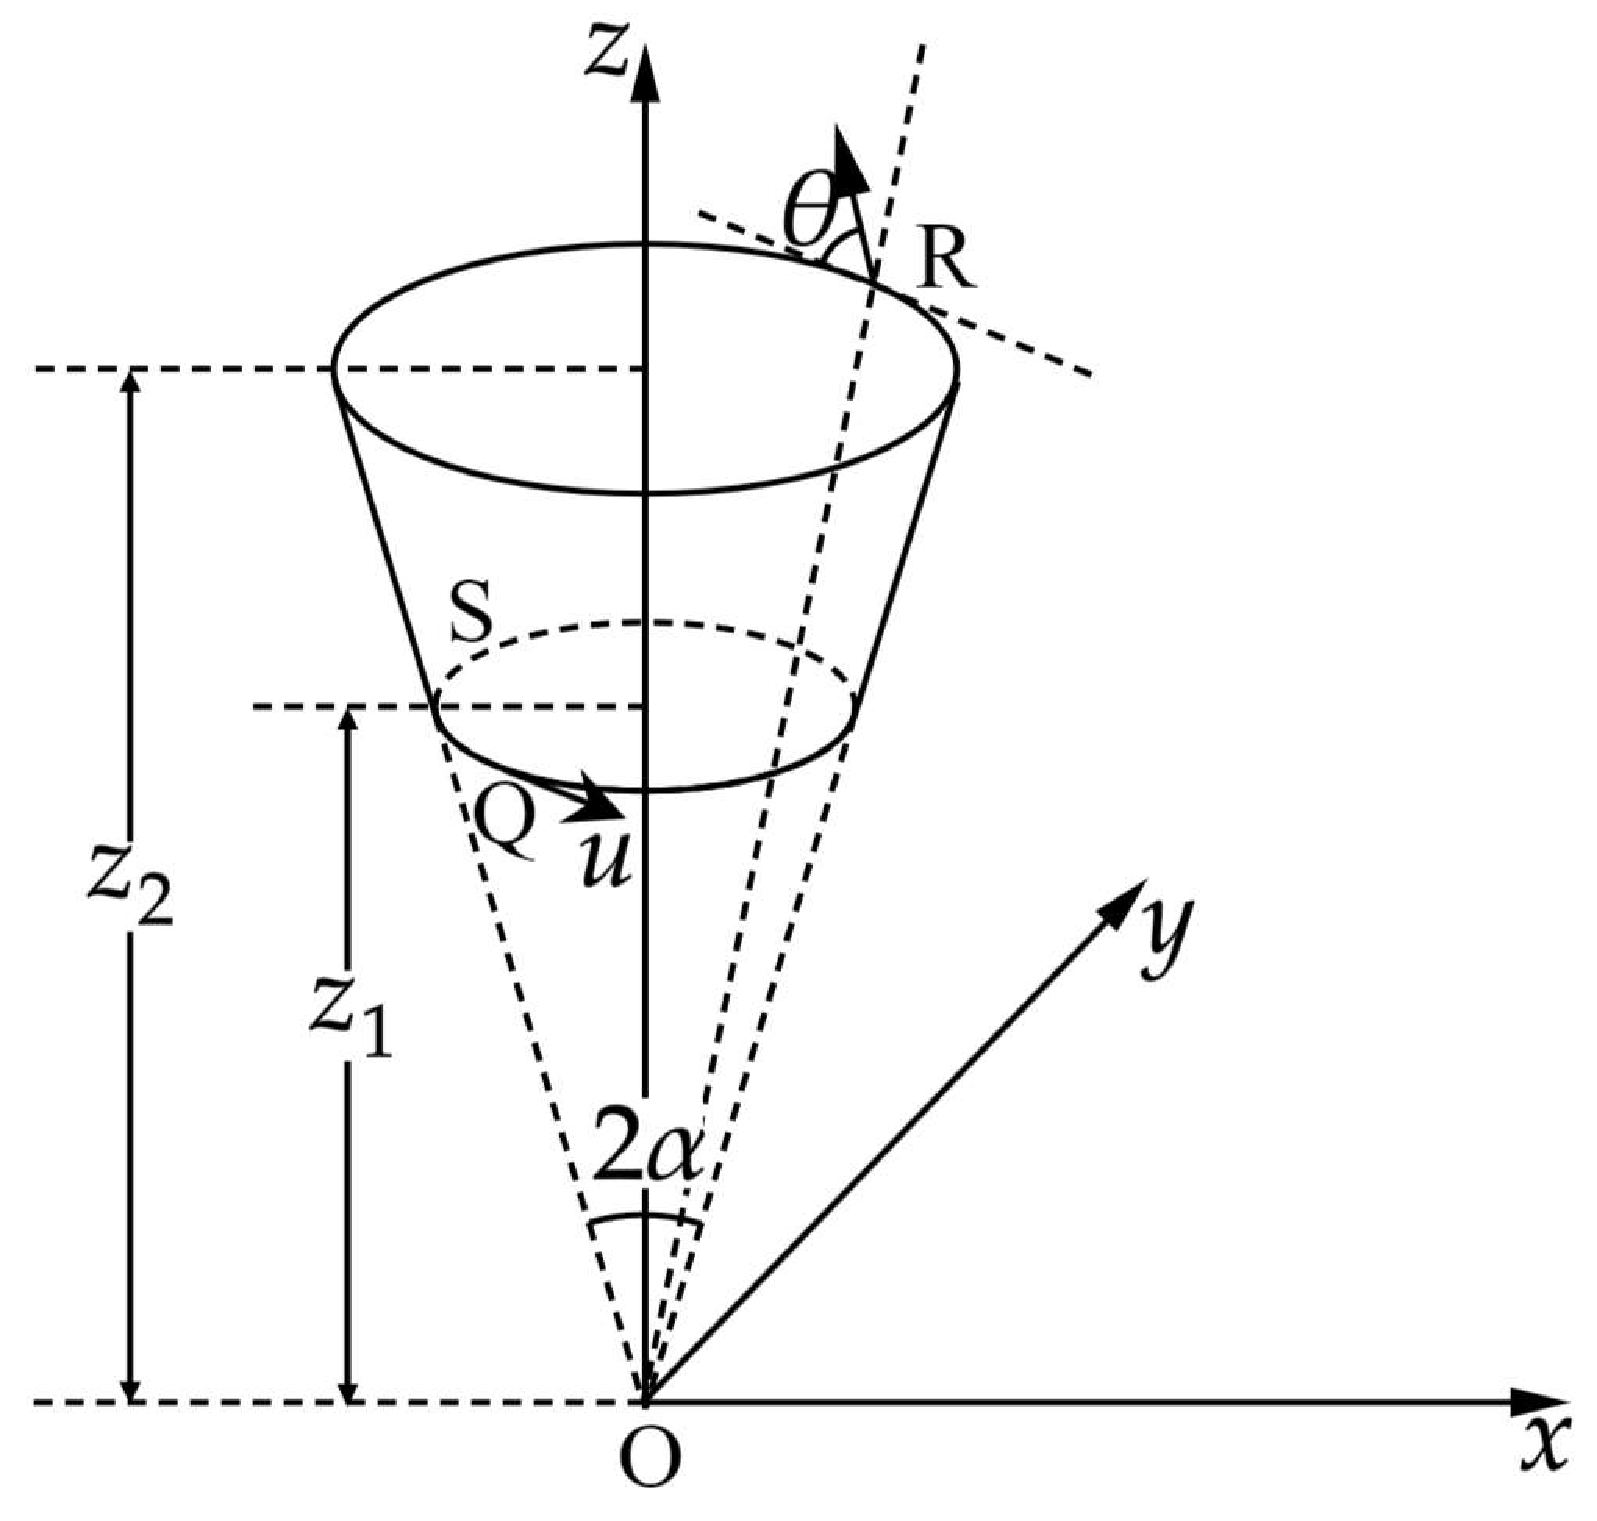
\includegraphics[width=7cm]{fig/fig_1_8.pdf}
\end{figure}

\begin{enumerate}[I]
  \item {\hzw} 質点が$z = z_0\ (z_1 < z_0 < z_2)$の水平面内を等速円運動している.水平面内の等速円運動の運動方程式と鉛直方向の運動方程式とをそれぞれ書け.ただし,等速円運動の角速度を$\omega$,質点がSから受ける抗力の大きさを$N$とする.また,ここから$\omega$と$N$を求めよ.
  \item {\hzw}質点が水平面内を運動していない場合であっても,質点にはたらく力のベクトルを考えると,その水平成分は常に円錐の軸に向かっている.このため,質点を$xy$平面に投影してできる点の運動について,太陽の周りを回る惑星の運動と同様に面積速度一定の法則が成り立つ.この性質を利用して,Sの下端の円上の点Qから速さ$u$で円周に沿って打ち出された質点の運動を考える.
  \begin{enumerate}[(1)]
    \item {\hzw}質点を$xy$平面に投影してできる円の面積速度を求めよ.
    \item {\hzw}質点がSから外に飛び出すことなく運動し続けるためには$u$はどのような範囲になければならないかを答えよ.
    \item {\hzw}速度が前問の条件を満たさず,図に示すように上端のある点Rから質点が飛び出すとする.飛び出す瞬間の速度ベクトルと,Rにおける円の接線がなす角を$\theta$とする.速度ベクトルはRにおける円の接線と線分ORとを含む平面内であることに注意して$\cos\theta$を求めよ.
    \item {\hzw}前問で上端から飛び出した後に到達する最も高い点の$z$座標を求めよ.
  \end{enumerate}
\end{enumerate}
\end{document}